\documentclass[supplement,hidelinks]{siamart251216}
% Manuscript v9 in the SIAM article class (SISC submission).
\usepackage{amssymb,mathtools}
\usepackage{booktabs}
\usepackage{array}
\usepackage{enumitem}
\usepackage[protrusion=true,expansion=false]{microtype}
\usepackage{placeins}
\graphicspath{{../figures_v9/}}
\usepackage{bm}
\usepackage{textcomp}
\renewcommand{\topfraction}{0.95}
\renewcommand{\bottomfraction}{0.9}
\renewcommand{\textfraction}{0.05}
\renewcommand{\floatpagefraction}{0.65}
\ifpdf
\hypersetup{
 pdftitle={Supplementary Materials: Symbol-based residual certification of reduced and neural surrogates for tempered-fractional CGMY pricing},
 pdfauthor={D. Damircheli}}
\fi
\externaldocument[][nocite]{main_v9}
\newsiamremark{remark}{Remark}
\newsiamthm{assumption}{Assumption}
\headers{Symbol-based certification for CGMY pricing}{D. Damircheli}
\title{Symbol-based residual certification of reduced and neural surrogates for tempered-fractional CGMY pricing\thanks{Submitted to the editors DATE.}}
\author{Davood Damircheli\thanks{Department of Mathematics, Louisiana State University, Baton Rouge, LA 70803, USA
(\email{ddamircheli@lsu.edu}).}}
% ----------------------------- notation --------------------------
\newcommand{\R}{\mathbb{R}}
\newcommand{\Pset}{\mathcal{P}}
\newcommand{\Sop}{\mathcal{S}}
\newcommand{\Vh}{V_h^0}
\newcommand{\Vmu}{V_{\mu}}
\newcommand{\Vp}[1]{V_{#1}}
\newcommand{\Mh}{M_h}
\newcommand{\Ah}{A_h}
\newcommand{\Sh}{S_h}
\newcommand{\norm}[1]{\left\lVert #1\right\rVert}
\newcommand{\ip}[2]{\left\langle #1,#2\right\rangle}
\newcommand{\dt}{\Delta\tau}
\newcommand{\etaSharp}{\eta_{\mathrm{sh}}}
\newcommand{\etaMass}{\eta_{\mathrm{ms}}}
\newcommand{\etaGuar}{\eta_{\mathrm{gu}}}
\newcommand{\ee}{\mathbf e}
\newcommand{\cc}{\mathbf c}
\newcommand{\rr}{\bm\rho}
\newcommand{\ff}{\mathbf f}
\newcommand{\vv}{\mathbf v}
\newcommand{\bb}{\mathbf b}
\newcommand{\zz}{\mathbf z}
\newcommand{\yy}{\mathbf y}
\newcommand{\ww}{\mathbf w}
\newcommand{\sres}{\mathbf s}
\newcommand{\dd}{\bm\delta}
\newcommand{\rf}{r}
\newcommand{\Hs}{H^{s_\mu}_{M,G}}
\newcommand{\Dm}{\mathcal D_G^-}
\newcommand{\Dp}{\mathcal D_M^+}
\newcommand{\Aop}{\mathcal A_\mu}
\DeclareMathOperator{\Real}{Re}
% ---------------------------- v9 macros ---------------------------
\newcommand{\Tn}[2]{T_{#1}(#2)}          % Toeplitz section T_n(f)
\newcommand{\sym}[1]{#1}                 % symbol (plain letter; change here to decorate)
\newcommand{\smin}{s_{\min}}
\newcommand{\Thmu}{\Theta_\mu}
\newcommand{\todo}[1]{\textcolor{red!70!black}{[\textbf{TODO:} #1]}}

\begin{document}
\maketitle
\section{Explicit constants and proof of uniform stability}
\label{app:proof-uniform}\label{ssec:lk-coercivity}
For the box \eqref{eq:parameter-set}, define
\begin{equation}
  a_\ast:=\max\{M_{\max},G_{\max}\},\quad
  \kappa_Y:=\frac{2e^{-\pi}}{(2-Y)\pi^{Y}},\quad
  \Theta_w:=\max\{1,M_{\max}^2,G_{\max}^2\}^{Y_{\max}/2}.
  \label{eq:uniform-constants-aux}
\end{equation}
Explicit admissible choices are
\begin{equation}
  c_1
  =\min_{\mu\in\Pset}\min\Bigl\{
    \frac{\rf}{1+2^{1+Y/2}a_\ast^{Y}},\;
    \frac{C\,\kappa_Y}{2^{Y/2}}
  \Bigr\}
  =\frac{r_{\min}}{1+2^{1+Y_{\max}/2}a_\ast^{Y_{\max}}},
  \label{eq:c1-explicit}
\end{equation}
the second branch being larger on the box of equation~(\ref{eq:numerical-box}) of the main text, and
\begin{equation}
  C_{\rm cont}
  =2\Bigl(
    \Omega_\ast
    +2C_{\max}\gamma_{\max}\max\{1,a_\ast^2\}^{Y_{\max}/2}
    +\lambda_\ast
  \Bigr),
  \label{eq:Ccont-explicit}
\end{equation}
where
\begin{equation}
\begin{gathered}
\gamma_{\max}:=\!\!\max_{Y\in[Y_{\min},Y_{\max}]}\!\!\Gamma(-Y)<\infty,
\qquad
\Omega_\ast:=\sup_{\mu\in\Pset}|\rf-\omega_S(\mu)|,
\qquad
\lambda_\ast:=\sup_{\mu\in\Pset}\lambda_0(\mu),
\end{gathered}
\label{eq:uniform-aux-constants}
\end{equation}
the last two being finite.
Throughout, $\mu=(C,G,M,Y,\rf)\in\Pset$ and $s_\mu=Y/2\in(1/2,1)$.  We work on
the full line and transfer to $\Omega$ at the end using
the zero-extension convention
\eqref{eq:energy-space}, which preserves all constants.
\medskip\noindent
\textbf{Step 1: uniform equivalence of the parameter-dependent norm.}
Let $s\in[Y_{\min}/2,Y_{\max}/2]\subset(1/2,1)$ and let
$w_\mu(\xi):=1+|M-i\xi|^{2s}+|G+i\xi|^{2s}
=1+(M^2+\xi^2)^{s}+(G^2+\xi^2)^{s}$ be the weight in
\eqref{eq:HMG-norm}.  Since $s\le1$ and $(a+b)^s\le a^s+b^s$ for $s\in(0,1]$,
\[
  w_\mu(\xi)\ \le\ 1+2\max\{1,M_{\max}^2,G_{\max}^2\}^{s}(1+\xi^2)^{s}
  \ \le\ (1+2\Theta_w)(1+\xi^2)^{s},
\]
with $\Theta_w=\max\{1,M_{\max}^2,G_{\max}^2\}^{Y_{\max}/2}$, using
$(1+\xi^2)^s\ge1$.  For the lower bound, $w_\mu(\xi)\ge1+|\xi|^{2s}$ and,
since $(1+\xi^2)^s\le2^s\max\{1,|\xi|^{2s}\}\le2(1+|\xi|^{2s})$ for
$s\le1$,
\[
  w_\mu(\xi)\ \ge\ \tfrac12(1+\xi^2)^{s}.
\]
Hence, uniformly in $\mu\in\Pset$,
\begin{equation}
  \tfrac12\norm{u}_{H^{s_\mu}(\R)}^2
  \ \le\ \norm{u}_{H^{s_\mu}_{M,G}(\R)}^2
  \ \le\ (1+2\Theta_w)\norm{u}_{H^{s_\mu}(\R)}^2 ,
  \label{eq:uniform-norm-equivalence}
\end{equation}
where $\norm{u}_{H^{s}(\R)}^2=\tfrac1{2\pi}\int(1+\xi^2)^{s}|\widehat u|^2$.

\medskip\noindent
\textbf{Step 2: uniform continuity.}
From \eqref{eq:symbol}, for every $\xi$,
\[
  |A_\mu(\xi)|
  \le|\rf-\omega_S||\xi|
   +C\Gamma(-Y)\bigl[(M^2+\xi^2)^{Y/2}+(G^2+\xi^2)^{Y/2}\bigr]
   +\lambda_0 .
\]
The map $(C,G,M,Y)\mapsto\omega_S$ of \eqref{eq:martingale-correction} is
continuous on $\Pset$ because $(M-1)^Y$ is continuous and finite on the selected box
(and remains so at $M=1$), and $\Gamma(-Y)$ is continuous on $[Y_{\min},Y_{\max}]\subset(1,2)$;
hence $\Omega_\ast<\infty$ and $\lambda_\ast<\infty$.  Since $Y>1$ we have
$|\xi|\le(1+\xi^2)^{Y/2}$, and
$(a^2+\xi^2)^{Y/2}\le\max\{1,a^2\}^{Y/2}(1+\xi^2)^{Y/2}$.  Therefore
\begin{equation}
  |A_\mu(\xi)|
  \le\Bigl(\Omega_\ast+2C_{\max}\gamma_{\max}\max\{1,a_\ast^2\}^{Y_{\max}/2}
   +\lambda_\ast\Bigr)(1+\xi^2)^{s_\mu}.
  \label{eq:uniform-symbol-upper}
\end{equation}
By Plancherel's theorem and the Cauchy--Schwarz inequality,
\[
  |a_\R(u,w)|
  \le\Bigl(\sup_{\xi\in\R}\frac{|A_\mu(\xi)|}{(1+\xi^2)^{s_\mu}}\Bigr)
  \norm{u}_{H^{s_\mu}(\R)}\norm{w}_{H^{s_\mu}(\R)},
\]
and
\eqref{eq:uniform-norm-equivalence} converts the $H^{s_\mu}$ norms into
$H^{s_\mu}_{M,G}$ norms at the cost of a factor $2$.  This gives
\eqref{eq:Ccont-explicit}.


\medskip\noindent
\textbf{Step 3: the L\'evy--Khintchine form.}
By Lemma~\ref{lem:LK},
\begin{equation}
  \Real A_\mu(\xi)=\rf+C\,[I_G(\xi)+I_M(\xi)],\qquad
  I_a(\xi)=\int_0^\infty(1-\cos\xi x)\,e^{-ax}x^{-1-Y}dx\ \ge0,
  \label{eq:uniform-low-freq}
\end{equation}
so $\Real A_\mu(\xi)\ge \rf\ge r_{\min}>0$ for all $\xi$; the drift term is purely
imaginary and does not enter.  (This is where $r_{\min}>0$ is used.)  Two elementary
lower bounds for $I_a$ follow from $1-\cos u\ge 2u^2/\pi^2$ on $|u|\le\pi$: restricting the
integral to $0<x\le\pi/|\xi|$ and substituting $u=ax$,
\begin{equation}
  I_a(\xi)\ \ge\ \frac{2\xi^2}{\pi^2}\,a^{Y-2}\!\int_0^{a\pi/|\xi|}\!u^{1-Y}e^{-u}\,du
  \ \ge\ \frac{2}{\pi^2}\,\gamma_Y\,a^{Y-2}\xi^2\quad(|\xi|\le a),
  \label{eq:LK-low}
\end{equation}
with $\gamma_Y:=\int_0^\pi u^{1-Y}e^{-u}\,du$, and, bounding $e^{-ax}\ge e^{-\pi}$ on $0<x\le\pi/|\xi|$ when $|\xi|\ge a$,
\begin{equation}
  I_a(\xi)\ \ge\ e^{-\pi}\frac{2\xi^2}{\pi^2}\int_0^{\pi/|\xi|}x^{1-Y}dx
  =\frac{2e^{-\pi}}{(2-Y)\pi^{Y}}\,|\xi|^{Y}=\kappa_Y|\xi|^Y\quad(|\xi|\ge a).
  \label{eq:LK-high}
\end{equation}
Both bounds hold for every $Y\in(0,2)$; the hypothesis $Y>1$ is needed only to
control the drift by the $H^{Y/2}$ norm in Step~2.

\medskip\noindent
\textbf{Step 4: the weight.}
The weight of \eqref{eq:HMG-norm} with $q=s_\mu=Y/2$ is
$w_\mu(\xi)=1+(M^2+\xi^2)^{Y/2}+(G^2+\xi^2)^{Y/2}$.  Since
$(a^2+\xi^2)^{Y/2}\le 2^{Y/2}\max\{a,|\xi|\}^{Y}$,
\begin{equation}
  w_\mu(\xi)\le 1+2^{1+Y/2}a_\ast^{Y}\quad(|\xi|\le a_\ast),\qquad
  w_\mu(\xi)\le 1+2^{1+Y/2}|\xi|^{Y}\quad(|\xi|\ge a_\ast).
  \label{eq:weight-bounds}
\end{equation}

\medskip\noindent
\textbf{Step 5: combination.}
For $|\xi|\le a_\ast$, \eqref{eq:uniform-low-freq} and \eqref{eq:weight-bounds} give
$\Real A_\mu(\xi)\ge \rf\,(1+2^{1+Y/2}a_\ast^{Y})^{-1}w_\mu(\xi)$.
For $|\xi|\ge a_\ast\ge\max\{G,M\}$, \eqref{eq:LK-high} applies to both $I_G$ and $I_M$, so
$\Real A_\mu(\xi)\ge \rf+2C\kappa_Y|\xi|^Y$, and with \eqref{eq:weight-bounds} and
$(\alpha+\beta)/(\gamma+\delta)\ge\min\{\alpha/\gamma,\beta/\delta\}$,
\[
  \frac{\Real A_\mu(\xi)}{w_\mu(\xi)}\ \ge\ \min\Bigl\{\rf,\ \frac{2C\kappa_Y}{2^{1+Y/2}}\Bigr\}
  \ \ge\ \min\Bigl\{\frac{\rf}{1+2^{1+Y/2}a_\ast^{Y}},\ \frac{C\kappa_Y}{2^{Y/2}}\Bigr\}.
\]
Hence $\Real A_\mu(\xi)\ge c_1\,w_\mu(\xi)$ for all $\xi$ with $c_1$ as in
\eqref{eq:c1-explicit}, and Plancherel's theorem gives
$\Real a_\R(u,u)\ge c_1\norm{u}_{H^{s_\mu}_{M,G}(\R)}^2$ directly in the weighted norm,
without the equivalence factor of Step~1.

\medskip\noindent
\textbf{Step 6: transfer to $\Omega$.}
For $v,w\in\Vmu$ the zero extensions satisfy
$\widetilde v,\widetilde w\in H^{s_\mu}(\R)$ with
$\norm{\widetilde v}_{L^2(\R)}=\norm{v}_{L^2(\Omega)}$, and by definition
$a_\mu(v,w)=a_\R(\widetilde v,\widetilde w)$ and
$\norm{v}_{\Vmu}=\norm{\widetilde v}_{H^{s_\mu}_{M,G}(\R)}$.  Both estimates
therefore transfer with identical constants, independent of $h$ and of
$\Omega$.  Finally, for real-valued $v$ the form $a_\mu(v,v)$ is real, so
$a_\mu(v,v)=\Real a_\mu(v,v)$.  \qed


The constants are explicit admissible choices rather than optimal ones.
On the box of equation~(\ref{eq:numerical-box}) of the main text, $c_1=5.11\times10^{-5}$ (attained at
$Y=Y_{\max}$, $\rf=r_{\min}$, $a_\ast=M_{\max}=9$) and $C_{\rm cont}\approx2.5\times10^3$.
The infimum of $\Real A_\mu(\xi)/w_\mu(\xi)$ over the box is in fact attained at $\xi=0$, where
\eqref{eq:uniform-low-freq} is an equality: its value $r_{\min}/(1+M_{\max}^{Y_{\max}}+G_{\max}^{Y_{\max}})
=1.40\times10^{-4}$ is confirmed numerically over $544$ box points and $\xi\in[0,10^6]$
(\texttt{results/coercivity\_c1.json}), so the explicit constant is within a factor three of the
optimal one.  The earlier version of this appendix obtained $c_1\approx1.6\times10^{-8}$ from a
high-frequency argument that required $Y_{\min}>1$ at every step; the L\'evy--Khintchine form
removes both the loss and that requirement from the coercivity part of the proof.

\section{Exact-assembly consequences and constrained dual norms}
\label{ssec:exact-assembly}
Under exact assembly, $z^\top\Sh z=a_\mu(z_h,z_h)$, so uniform coercivity
implies $\Sh\succ0$. The symmetric parts of $\Mh+\dt\Ah/2$ and
$\Mh+\dt\Ah$ are positive definite, giving nonsingularity.
\begin{lemma}[Positive-rate mass lower bound for exact assembly]
\label{lem:mass-lower}
Under exact assembly (Section~\ref{ssec:exact-assembly}), for
$\mu\in\Pset$ (so $\rf>0$),
\begin{equation}
  \Sh(\mu)\succeq \rf\,\Mh
  \label{eq:S-ge-rM}
\end{equation}
in the Loewner order, and consequently
\begin{equation}
  \bb^\top\Sh(\mu)^{-1}\bb\le \rf^{-1}\,\bb^\top\Mh^{-1}\bb
  \qquad\text{for every }\bb\in\R^{N_h}.
  \label{eq:mass-upper}
\end{equation}
\end{lemma}

\begin{proof}
By Lemma~\ref{lem:periodisation} and Plancherel's theorem,
\[
  \zz^\top\Sh\zz=a_\mu(z_h,z_h)=a_\R(\widetilde z_h,\widetilde z_h)
  =\frac1{2\pi}\int_\R\Real A_\mu(\xi)\,\bigl|\widehat{\widetilde z_h}(\xi)\bigr|^2\,d\xi .
\]
The exact symbol identity of \cite{DamircheliCGMY2026}, namely
\begin{equation}
\Real A_\mu(\xi)
=\rf+C\Gamma(-Y)\Bigl[\bigl(M^Y-\Real(M-i\xi)^Y\bigr)
+\bigl(G^Y-\Real(G+i\xi)^Y\bigr)\Bigr],
\label{eq:symbol-real-exact}
\end{equation}
together with $\Gamma(-Y)>0$ for $Y\in(1,2)$ and the monotonicity
$\Real(a\pm i\xi)^Y\le a^Y$, gives $\Real A_\mu(\xi)\ge \rf$ for all $\xi$.  Hence
\[
  \zz^\top\Sh\zz\ \ge\ \rf\norm{\widetilde z_h}^2_{L^2(\R)}
  =\rf\norm{z_h}^2_{L^2(\Omega)}=\rf\,\zz^\top\Mh\zz .
\]
Inversion of the Loewner
inequality between positive definite matrices reverses it, giving
\eqref{eq:mass-upper}.
\end{proof}
Exact assembly also implies the mesh-uniform bound on $\kappa_h$:
\[
 \|\Ah v\|_{\Sh^{-1}}
 =\sup_{w\ne0}\frac{a_\mu(v_h,w_h)}{\|w\|_{\Sh}}
 \le\frac{C_{\rm cont}}{c_1}\|v\|_{\Sh}.
\]
For any assembled matrix with SPD symmetric part, duality gives
$\|\Ah v\|_{\Sh^{-1}}\ge v^\top\Ah v/\|v\|_{\Sh}=\|v\|_{\Sh}$,
proving $\kappa_h\ge1$. This quantity is an operator norm, rather than the
condition number of $\Sh$.
\begin{proposition}[Conservatism of a full-space dual norm]
\label{prop:full-space-conservative}
Suppose $\bar S\succ0$, and the reference and candidate have identical
prescribed coefficients. Then $S_I\succ0$ and
\begin{equation}
 \rho_I^\top S_I^{-1}\rho_I
 \le (E\rho_I)^\top\bar S^{-1}(E\rho_I).
 \label{eq:full-space-conservative}
\end{equation}
Consequently a valid upper Riesz bracket for the zero-padded free residual
using $\bar S$ is also a conservative reliability bound for the constrained
problem, subject to the same initial-error and arithmetic assumptions.
\end{proposition}
\begin{proof}
The dual quadratic form equals
$\sup_v(2r^\top v-v^\top S v)$. Restricting the full-space supremum to
$v=Ew$ yields the free-space supremum, proving
\eqref{eq:full-space-conservative}. Positive definiteness restricts to every
principal subspace.
\end{proof}
The converse positivity implication fails because prescribed directions
can make $\bar S$ indefinite while $S_I$ is positive. The entire residual,
Riesz action and spectral bound must use the same constrained space.

\section{Discrete parameter stability}
\label{ssec:solution-operator}
\begin{proposition}[Discrete parameter stability of the solution map]
\label{prop:discrete-lipschitz}
Fix a mesh, a time grid, and a payoff $\psi$; the assembled symmetric
matrix $\Sh(\mu_1)$ is positive definite by Theorem~\ref{thm:spectral}. Let
$\mu_1,\mu_2\in\Pset$
with $\cc_h(\mu_1),\cc_h(\mu_2)$ the corresponding Crank--Nicolson
trajectories of \eqref{eq:cn-reference}.  Then, for every
$m=1,\dots,N_T$,
\begin{equation}
\begin{aligned}
  \norm{\cc_h^m(\mu_1)-\cc_h^m(\mu_2)}_{\Mh}^2
  \le{}& \norm{\cc_h^0(\mu_1)-\cc_h^0(\mu_2)}_{\Mh}^2\\
  &+\dt\sum_{n=0}^{m-1}
  \bigl\lVert\bm\varrho^{\,n+1/2}\bigr\rVert_{\Sh(\mu_1)^{-1}}^2 ,
\end{aligned}
  \label{eq:discrete-lipschitz}
\end{equation}
where the parameter-perturbation residual is
\begin{equation}
  \bm\varrho^{\,n+1/2}
  :=\bigl(\Ah(\mu_1)-\Ah(\mu_2)\bigr)\overline\cc_h^{\,n+1/2}(\mu_2)
   -\bigl(\overline\ff^{\,n+1/2}(\mu_1)-\overline\ff^{\,n+1/2}(\mu_2)\bigr).
  \label{eq:param-residual}
\end{equation}
Under exact assembly of the conforming variational matrices,
Theorem~\ref{thm:uniform-coercivity} additionally gives
\begin{equation}
  \norm{\bigl(\Ah(\mu_1)-\Ah(\mu_2)\bigr)\vv}_{\Sh(\mu_1)^{-1}}
  \le
  \frac{1}{c_1}\,
  \sup_{0\ne v_h,w_h\in\Vh}
  \frac{|a_{\mu_1}(v_h,w_h)-a_{\mu_2}(v_h,w_h)|}
       {\norm{v_h}_{\Vp{\mu_1}}\norm{w_h}_{\Vp{\mu_1}}}\,
  \norm{\vv}_{\Sh(\mu_1)},
  \label{eq:matrix-difference}
\end{equation}
so a bound on the difference of the two bilinear forms in a \emph{single}
norm---that of $\mu_1$---suffices, and no common energy space is needed.
\end{proposition}

\begin{proof}
The difference $\ee^n:=\cc_h^n(\mu_1)-\cc_h^n(\mu_2)$ satisfies the
Crank--Nicolson error equation \eqref{eq:discrete-error-equation} with
$\rr_\theta^{n+1/2}$ replaced by $\bm\varrho^{\,n+1/2}$ of
\eqref{eq:param-residual}, since $\cc_h(\mu_2)$ solves the $\mu_2$ scheme
exactly.  Apply Theorem~\ref{thm:fully-discrete-certificate} with
$\Sh=\Sh(\mu_1)$.  Estimate \eqref{eq:matrix-difference} follows from
the continuity argument above applied to the bilinear form
$a_{\mu_1}-a_{\mu_2}$.
\end{proof}
This fixed-grid statement compares both trajectories in the norm of the
first parameter. A continuum regularity result across varying $Y$ would
require additional control of the changing energy spaces.

\section{Other time schemes and exponential shifts}
\label{ssec:semidiscrete}\label{ssec:be-certificate}\label{ssec:shifted}
The following extensions follow the same energy argument as
Theorem~\ref{thm:fully-discrete-certificate}.
For a differentiable candidate and a semidiscrete reference, define
$\rho=\Mh\dot\cc_\theta+\Ah\cc_\theta-\ff$. Then
\begin{equation}
 \|\ee(t)\|_{\Mh}^2+\int_0^t\|\ee\|_{\Sh}^2
 \le\|\ee(0)\|_{\Mh}^2+\int_0^t\|\rho\|_{\Sh^{-1}}^2.
 \label{eq:semidiscrete-certificate}
\end{equation}
Multiply the error equation by $\ee^\top$, apply Young's inequality, and
integrate.
For backward Euler, the residual is
$\rho^{n+1}=\Mh(c_\theta^{n+1}-c_\theta^n)/\dt_n
+\Ah c_\theta^{n+1}-f^{n+1}$ and
\begin{equation}
 \|\ee^{n+1}\|_{\Mh}^2+\|\ee^{n+1}-\ee^n\|_{\Mh}^2
 +\dt_n\|\ee^{n+1}\|_{\Sh}^2
 \le\|\ee^n\|_{\Mh}^2+\dt_n\|\rho^{n+1}\|_{\Sh^{-1}}^2.
 \label{eq:be-certificate}
\end{equation}
This follows from
$2y^\top\Mh(y-z)=\|y\|_{\Mh}^2-\|z\|_{\Mh}^2+\|y-z\|_{\Mh}^2$.
A Rannacher start combines backward-Euler half steps with CN
\cite{Rannacher1984}; summing the corresponding bounds, with the initial
term retained, gives the certificate for the mixed trajectory.
Each step must use its own scheme's residual.

For an exact-assembly G\aa rding bound
$a_\mu(v,v)\ge c_1\|v\|_{V_\mu}^2-c_2\|v\|_{L^2}^2$, choose
$\sigma>c_2$ and set
$A_\sigma=\Ah+\sigma\Mh$, $S_\sigma=\Sh+\sigma\Mh$.
Then $S_\sigma\succeq(\sigma-c_2)\Mh$.
Advance $d_h$ by CN for the shifted operator with forcing
$g^n=e^{-\sigma\tau_n}f^n$, and reconstruct
$c_{h,\sigma}^n=e^{\sigma\tau_n}d_h^n$.
For $d_\theta^n=e^{-\sigma\tau_n}c_\theta^n$ and its shifted CN residual
$\rho_\sigma$, the same theorem yields
\[
 \max_m\|c_{h,\sigma}^m-c_\theta^m\|_{\Mh}
 \le e^{\sigma T}
 \left(\|d_h^0-d_\theta^0\|_{\Mh}^2+
 \dt\sum_n\|\rho_\sigma^{n+1/2}\|_{S_\sigma^{-1}}^2\right)^{1/2}.
\]
This certifies the reconstructed shifted target. Exponential transformation
and CN discretisation do not commute, so it is a different discrete
trajectory from unshifted CN. The numerical studies use unshifted CN with
positive rates.

\section{Derivative bounds and continuum error separation}
\label{ssec:derivatives}\label{ssec:total-error}
For an $H^2(\Omega)$ spline space (cardinal order $p\ge3$), define the matrices
$R_h^{(j)}=((\phi_{h,k'}^{(j)},\phi_{h,k}^{(j)}))$ and the constants
$\Lambda_j=\lambda_{\max}(R_h^{(j)},\Mh)$ for $j=1,2$.
Since the common lifting cancels,
\[
 \|\partial_x^j(V_h^m-V_{\theta,h}^m)\|_{L^2}
 \le\sqrt{\Lambda_j}\eta_{\rm aug},
 \qquad \Lambda_j=O(h^{-2j}).
\]
Indeed, $\ee^\top R_h^{(j)}\ee\le\Lambda_j\ee^\top\Mh\ee$.
With the Greeks $\Delta=e^{-x}V_x$ and $\Gamma_{\rm opt}=e^{-2x}(V_{xx}-V_x)$,
\[
 \|\Delta_h-\Delta_\theta\|_{L^2}
 \le e^{-x_{\min}}\sqrt{\Lambda_1}\eta_{\rm aug},\qquad
 \|\Gamma_{{\rm opt},h}-\Gamma_{{\rm opt},\theta}\|_{L^2}
 \le e^{-2x_{\min}}(\sqrt{\Lambda_2}+\sqrt{\Lambda_1})\eta_{\rm aug}.
\]
These global factors can be conservative on a wide log-price domain and
grow under refinement. A rigorous numerical supremum of the point factor
in \eqref{eq:gamma-infty} requires validated cellwise extrema.

Under exact assembly, the regularity and buffer assumptions of
\cite{DamircheliCGMY2026}, and an identical prescribed smooth lifting,
\begin{equation}
 \max_n\|V(\tau_n)-V_h^n\|_{L^2(\Omega)}
 \le C_\mu(h^{p-Y/2}+\dt^2+\varepsilon_b).
 \label{eq:deterministic-error}
\end{equation}
The lifting discrepancies vanish because it is prescribed identically.
Combining this estimate with \eqref{eq:total-error-split} gives
\[
 \|V(\tau_m)-V_{\theta,h}^m\|_{L^2}
 \le C_\mu(h^{p-Y/2}+\dt^2+\varepsilon_b)+\eta_{\rm aug}.
\]
The deterministic constants and buffer error are not evaluated as
computable bounds here; the first term is assessed instead by the price comparison of
Section~\ref{ssec:calibration}, and the certificate supplies the second.

\section{Residual certificate for the American put}
\label{ssec:vi}
% Theorem 6.1 of the note: residual certificate for the discrete variational inequality
For a discrete obstacle problem in coefficient space (B-splines are
nonnegative, so $c\ge\psi_h$ coefficientwise implies $U_h\ge\psi_h$), one
backward-Euler step reads: find $u^{n+1}\ge\psi_h$ with
$(B_+u^{n+1}-b^n)^\top(v-u^{n+1})\ge0$ for all $v\ge\psi_h$, where
$B_+=\Mh+\dt\Ah$ and $b^n=\Mh u^n+\dt f^{n+1}$.
\begin{theorem}[Residual certificate for the discrete variational inequality]
\label{thm:vi}
Let $\{u_\theta^n\}$ be any candidate with $u_\theta^n\ge\psi_h$ for all $n$,
let $R^n:=B_+u_\theta^{n+1}-\Mh u_\theta^n-\dt f^{n+1}$, and split
$R^n=R^n_+-R^n_-$ into positive and negative parts.  Then for every $m$,
\[
 \norm{e^m}_{\Mh}^2+\dt\sum_{n<m}\norm{e^{n+1}}_{\Sh}^2
 \ \le\ \norm{e^0}_{\Mh}^2
 +\sum_{n<m}\Bigl[\,2\,(R^n_+)^\top(u_\theta^{n+1}-\psi_h)
 +\dt^{-1}\norm{R^n_-}_{\Sh^{-1}}^2\Bigr].
\]
\end{theorem}
\begin{proof}
Test the inequality with $v=u_\theta^{n+1}$:
\[
(B_+e^{n+1}-\Mh e^n,\,e^{n+1})\le-(R^n,e^{n+1})=(R^n,u_\theta^{n+1}-u^{n+1}).
\]
Since $u^{n+1}\ge\psi_h$ and $R_+\ge0$, $(R^n_+,u_\theta^{n+1}-u^{n+1})\le(R^n_+,u_\theta^{n+1}-\psi_h)$,
and $(R^n_-,e^{n+1})\le\norm{R^n_-}_{\Sh^{-1}}\norm{e^{n+1}}_{\Sh}$.  The left side equals
\[
\tfrac12\bigl(\norm{e^{n+1}}_{\Mh}^2-\norm{e^n}_{\Mh}^2+\norm{e^{n+1}-e^n}_{\Mh}^2\bigr)+\dt\norm{e^{n+1}}_{\Sh}^2;
\]
Young's inequality and summation finish the proof.
\end{proof}
Everything in Sections~\ref{sec:galerkin}--\ref{sec:affine} (exact assembly, $\smin$, the banded norm,
the affine $A_Q$) applies verbatim; only the right-hand side gains the
complementarity term, which vanishes where the candidate is either off the
obstacle with nonpositive residual or on it.  The Crank--Nicolson version
requires testing the inequality at the midpoint, which is not admissible in
general; this is the one open technical point and the reason to use backward
Euler (or Rannacher-type restarts) for an American reference.

\section{Preconditioning and correction}
\label{ssec:correction-extension}
If $P_h\succ0$ and $\Sh\succeq\gamma_P P_h$ with $\gamma_P>0$, then
$r^\top\Sh^{-1}r\le\gamma_P^{-1}r^\top P_h^{-1}r$.
Alternatively $P_h$ can accelerate the Riesz iteration while the bracket
uses its independent bound on $\lambda_{\min}(\Sh)$.
\begin{proposition}[Contraction of a preconditioned correction]
\label{prop:correction-contraction}
Fix a time step and write the step equation as $B_+\zz=\bb$.  Let $P\succ0$ be
a preconditioner and consider the Richardson iteration
$\zz^{(i+1)}=\zz^{(i)}+P^{-1}(\bb-B_+\zz^{(i)})$ with residuals
$\sres^{(i)}=\bb-B_+\zz^{(i)}$.  Then
\begin{equation}
  \norm{\sres^{(i+1)}}_{P^{-1}}\le\rho_P\,\norm{\sres^{(i)}}_{P^{-1}},
  \qquad
  \rho_P:=\bigl\lVert I-P^{-1/2}B_+P^{-1/2}\bigr\rVert_2 .
  \label{eq:contraction}
\end{equation}
If $P=\Mh+\tfrac{\dt}{2}\Sh$, the symmetric part of $B_+$, then
\[
I-P^{-1/2}B_+P^{-1/2}=-\tfrac{\dt}{2}P^{-1/2}N_hP^{-1/2},\qquad N_h=\tfrac12(\Ah-\Ah^\top),
\]
with $N_h$ skew symmetric, so $\rho_P$ is determined entirely by the nonsymmetric part of the
CGMY operator and satisfies $\rho_P\le\tfrac{\dt}{2}\lVert P^{-1/2}N_hP^{-1/2}\rVert_2$.
\end{proposition}

\begin{proof}
$\sres^{(i+1)}=(I-B_+P^{-1})\sres^{(i)}$, so
$P^{-1/2}\sres^{(i+1)}=(I-P^{-1/2}B_+P^{-1/2})P^{-1/2}\sres^{(i)}$ and
\eqref{eq:contraction} follows by taking Euclidean norms.  For the second
claim, $B_+=P+\tfrac{\dt}{2}N_h$ by \eqref{eq:Sh} and the definition of $N_h$.
\end{proof}
The proposition proves contraction only when $\rho_P<1$; it is a
Richardson estimate and makes no contraction or timing assertion about the
GMRES correction used in the numerical experiments.
\FloatBarrier
\section{Verification of the assembly, the bounds and the solvers}
\label{sm:verification}
The studies of this section use the design of Section~\ref{ssec:design} of the main text (60 Crank--Nicolson
steps, several $N$); they verify the assembly of Section~\ref{ssec:assembly}, the bounds of
Theorems~\ref{thm:spectral} and~\ref{thm:comparison} and the solvers of Section~\ref{ssec:comparison}.
\subsection{Assembly verification}
Table~\ref{tab:assembly-v9} compares the assembled free matrix with the exact Galerkin matrix,
computed independently at 40 digits (alias series summed in closed form through Hurwitz zeta
tails, Toeplitz entries by a high-precision trapezoid rule).  The truncation error decreases
like $K^{-(2p-Y-1)}$ as predicted by Lemma~\ref{lem:tail}, and the bound $\varepsilon_K$ is
within a factor $1.1$--$3.7$ of the observed error at $K=100$ (at most $4.4$ at $K=20$ and $8.6$ at $K=5$).
\IfFileExists{../tables_v9/tab_assembly_v9.tex}{\begin{table}[!htbp]
\centering\small
\caption{Assembly verification against the exact Galerkin matrix (40-digit real-line fixture): relative operator-norm error of the free matrix $A_I$, median / max over the ten cost-study queries ($N\le256$; three at $N=512$). The principal-period rule (v8) is the alias sum with $K=0$; $\varepsilon_K/\|A_I\|_2$ is the bound of Lemma~\ref{lem:tail}.}
\label{tab:assembly-v9}
\begin{tabular}{rrrrrrr}
\toprule
$N$ & queries & principal period & $K=5$ & $K=20$ & $K=100$ & $\varepsilon_{100}/\|A_I\|_2$ (max)\\
\midrule
64 & 10 & 0.381 / 0.410 & $3.0\times10^{-5}$ / $5.8\times10^{-5}$ & $2.8\times10^{-7}$ / $7.7\times10^{-7}$ & $9.7\times10^{-10}$ / $4.2\times10^{-9}$ & $4.8\times10^{-9}$\\
128 & 10 & 0.370 / 0.408 & $2.5\times10^{-5}$ / $5.4\times10^{-5}$ & $2.3\times10^{-7}$ / $7.0\times10^{-7}$ & $8.1\times10^{-10}$ / $3.8\times10^{-9}$ & $4.4\times10^{-9}$\\
256 & 10 & 0.358 / 0.404 & $2.3\times10^{-5}$ / $5.1\times10^{-5}$ & $2.0\times10^{-7}$ / $6.6\times10^{-7}$ & $7.1\times10^{-10}$ / $3.6\times10^{-9}$ & $4.1\times10^{-9}$\\
512 & 3 & 0.333 / 0.402 & $1.6\times10^{-5}$ / $4.9\times10^{-5}$ & $1.2\times10^{-7}$ / $6.4\times10^{-7}$ & $3.6\times10^{-10}$ / $3.5\times10^{-9}$ & $4.0\times10^{-9}$\\
\bottomrule
\end{tabular}
\end{table}
}{\todo{Table pending (run\_E0.py E0.1)}}
\subsection{Spectral bound and comparison norm}
\begin{figure}[!htbp]
\centering
\IfFileExists{../figures_v9/F2_spectral_bound.pdf}{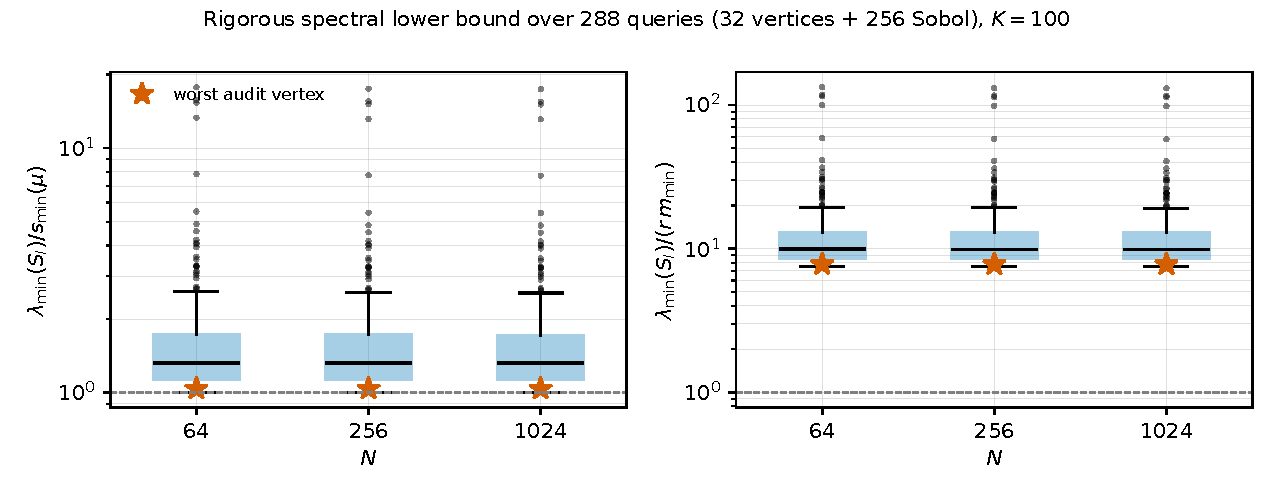
\includegraphics[width=0.94\linewidth]{F2_spectral_bound.pdf}}{\IfFileExists{../figures_v9/F2_spectral_bound.png}{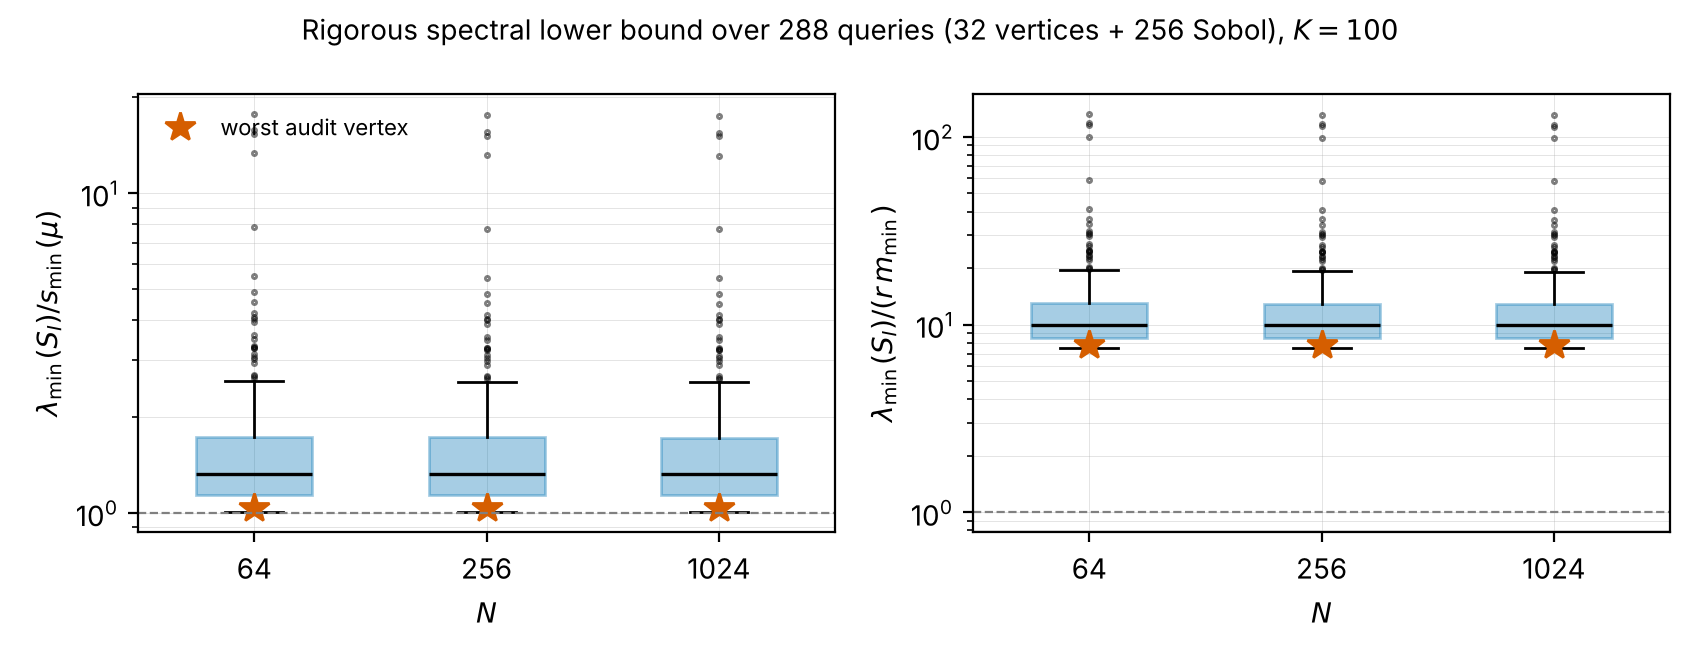
\includegraphics[width=0.94\linewidth]{F2_spectral_bound.png}}{\todo{figure F2 pending (run\_E0.py E0.2)}}}
\caption{Ratios $\lambda_{\min}(S_I)/\smin(\mu)$ (left) and $\lambda_{\min}(S_I)/(\rf m_{\min})$ (right)
over the 288 verification queries at $N=64,256,1024$; the star marks the worst vertex of the
earlier positivity audit.  Both ratios are $\ge1$ at every query, as Theorem~\ref{thm:spectral} asserts.}
\label{fig:spectral-bound}
\end{figure}
\begin{figure}[!htbp]
\centering
\IfFileExists{../figures_v9/F3_theta_and_effectivity.pdf}{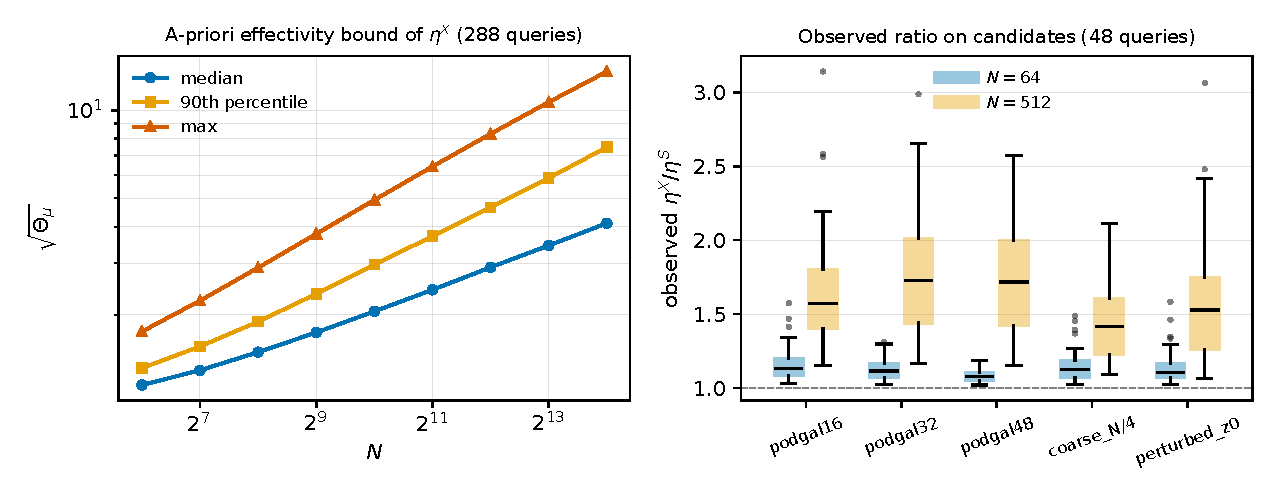
\includegraphics[width=0.94\linewidth]{F3_theta_and_effectivity.pdf}}{\IfFileExists{../figures_v9/F3_theta_and_effectivity.png}{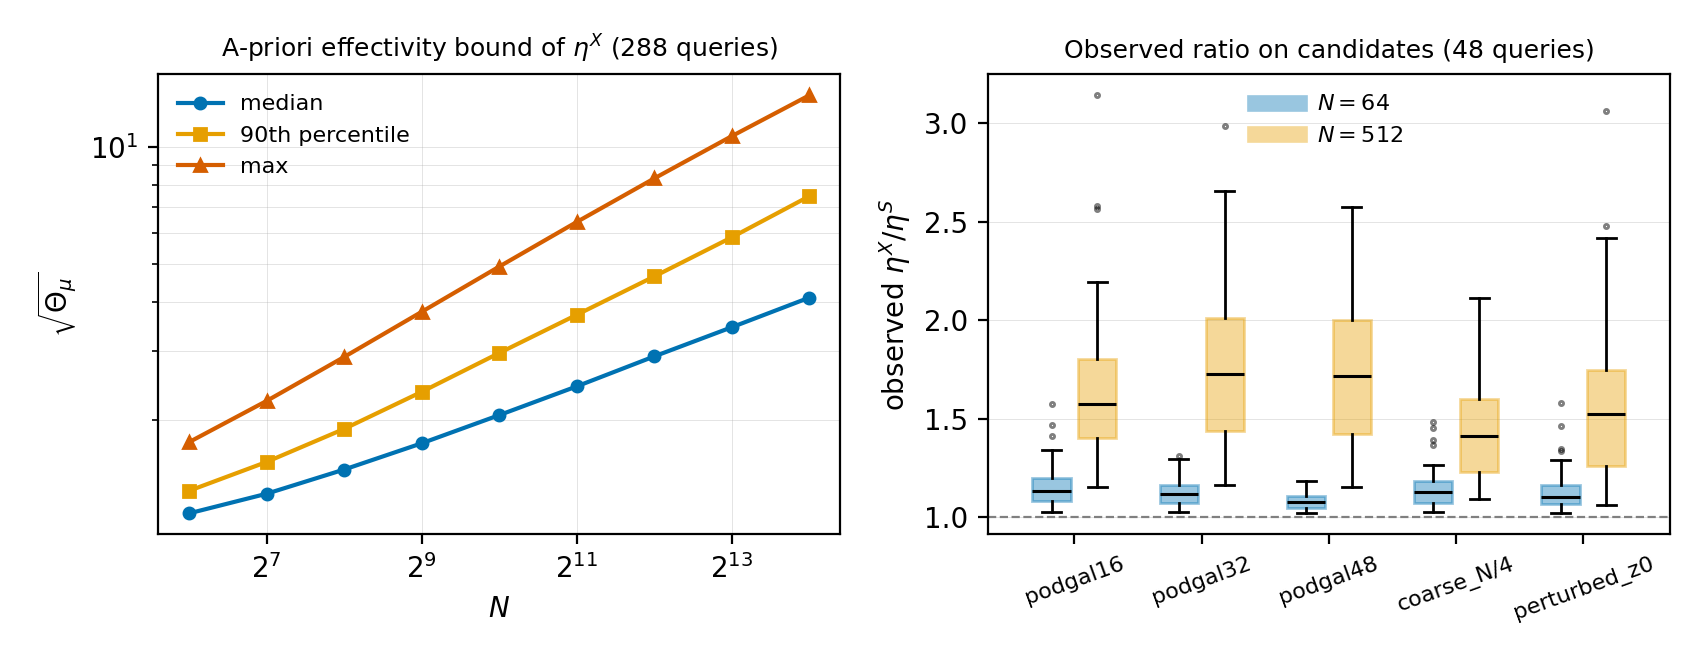
\includegraphics[width=0.94\linewidth]{F3_theta_and_effectivity.png}}{\todo{figure F3 pending (run\_E0.py E0.3)}}}
\caption{Left: the a-priori effectivity bound $\sqrt{\Thmu}$ of the banded certificate as a function of
$N$ (symbol only, 288 queries).  Right: observed ratio $\eta^X/\eta^S$ for POD--Galerkin candidates
(ranks 16, 32, 48), the prolonged coarse solution and exact dynamics from a perturbed initial vector,
at $N=64$ and $N=512$.}
\label{fig:theta}
\end{figure}
The bound of Theorem~\ref{thm:spectral} and the two-sided comparison \eqref{eq:comparison} hold at
all $289\times3$ tested (query, $N$) pairs (the 288 verification queries and the worst audit vertex); the generalised eigenvalues of $(S_I,X_I)$ lie in
$[1,\Thmu]$ in every case.  The a-priori factor $\sqrt{\Thmu}$ grows like
$(\min(G,M)h)^{(Y-2)/2}$ (median $1.15$, $1.74$, $2.05$, $2.91$, $4.11$ at $N=64$, $512$, $1024$,
$4096$, $16384$; maxima $1.75$, $3.78$, $4.93$, $8.30$, $13.6$), because the tempering scale moves
below the resolution of a degree-$(p-1)$ trigonometric minorant.  The observed ratio
$\eta^X/\eta^S$ on candidates is smaller: median $1.08$--$1.13$ at $N=64$ and $1.4$--$1.7$ at
$N=512$ (maximum $3.1$), so at the production resolution the banded certificate costs a factor
below two in effectivity; the production candidates of Section~\ref{ssec:e1} confirm the factor
$\eta^X/\eta^S\approx2$ at $N=1024$.
\subsection{Riesz solves and reference trajectories}
\IfFileExists{../tables_v9/tab_pcg_v9.tex}{\begin{table}[!htbp]
\centering\small
\caption{Iteration counts (median / max over 20 Sobol queries) to relative residual $10^{-12}$: conjugate gradients for the Riesz system $S_Iv=\rho$ with and without the circulant preconditioner built from the symbol samples, and circulant-preconditioned GMRES per Crank--Nicolson step for $B_+=M_I+\tfrac{\Delta\tau}{2}A_I$ (60 steps, warm start, mean over steps / max).}
\label{tab:pcg-v9}
\begin{tabular}{rrrr}
\toprule
$N$ & plain CG & circulant PCG & circulant GMRES ($B_+$)\\
\midrule
64 & 42 / 45 & 8 / 9 & 5.0 / 5\\
128 & 74 / 82 & 9 / 9 & 5.0 / 6\\
256 & 130 / 154 & 9 / 10 & 6.0 / 7\\
512 & 226 / 291 & 10 / 10 & 7.0 / 8\\
1024 & 384 / 548 & 10 / 11 & 7.1 / 12\\
2048 & 646 / 1025 & 11 / 11 & 8.0 / 13\\
4096 & 1078 / 1909 & 11 / 12 & 9.0 / 15\\
\bottomrule
\end{tabular}
\end{table}
}{\todo{Table pending (run\_E0.py E0.4)}}
Dense-LU and circulant-GMRES references agree to $10^{-12}$ in the $M_I$ norm for
$N\le1024$; the bracket width at convergence is below $10^{-20}$ relative for $N\le1024$ and
below $10^{-18}$ at $N=4096$, where it is set by the roundoff of the recomputed residual.
\subsection{Initial-error tests and \texorpdfstring{$Y<1$}{Y<1}}
On the 48 exact-dynamics cases with perturbed initial vectors ($\|\delta\|_{M_I}=10^{-4}$), both
$\eta^X_{\rm aug}$ and $\eta^S_{\rm aug}$ hold with effectivity $1.00\pm10^{-6}$, and the
residual-only estimators underestimate the error in every case.  For $Y\in\{0.5,0.8,0.95\}$
(same $C,G,M,\rf$ as the reference query) the bound $\alpha_{\rm lb}=0.0500=\rf$ is positive,
$\lambda_{\min}(S_I)\in[0.052,0.055]$, $\sqrt{\Thmu}\le1.5$, the preconditioned GMRES solve of
$B_+$ needs at most five iterations per step, and the certificate holds with effectivity one on
perturbed exact dynamics; the discrete framework therefore covers the finite-variation regime
without change.
\section{The neural-operator candidate of the earlier version}
\label{sm:deeponet}
The neural-operator candidate is a DeepONet with payoff and parameter branches and a time
trunk, latent dimension 64 and 80,002 trainable parameters, followed by a coefficient decoder
that supplies the spline-valued output. The experiments fix $\mathcal K=100$;
functional-input notation accommodates a payoff encoder but the benchmark
tests a parameter map for this single strike.  It was trained on the principal-period discretisation of the earlier version of this work, and
we did not retrain it on the exact-assembly references.  Certified as a candidate of the exact
system ($N=64$, $N_T=60$, 120 benchmark queries), it is rejected at every tolerance of the sweep
$10^{-3}\times\{0.1,\dots,10\}$: the median true error is $0.78$ (relative $3.1\times10^{-3}$), the
median exact bound $3.4$, with no false accept.  The certificate thus measures, correctly, the
distance between two discrete problems; the neural candidate of the production study is the
POD-NN below.
\section{Neural reduced candidates: results and training details}
\label{sm:training}
Table~\ref{tab:podnn} reports every POD-NN checkpoint of Section~\ref{ssec:e1} of the main text on
the 30 validation queries, and Table~\ref{tab:training} lists the optimiser, schedule, parameter
counts and wall times of the runs.
\IfFileExists{../tables_v9/tab_podnn_v9.tex}{\begin{table}[!htbp]
\centering\small
\caption{Neural reduced candidates (POD-NN, $r=48$) on the 30 validation queries at the production configuration: median true error and median augmented bounds of the three certificates, with the effectivity of the exact one. Standard output: $r\times N_T$ coefficients; space--time output: $r\times r_t$ coefficients of a temporal POD ($r_t=23$). Checkpoints selected by the validation median of the reduced certificate. The projection of the reference trajectories onto the same basis and the POD--Galerkin solution are the attainable floor. No candidate passes at $\varepsilon_N=1.18\times10^{-3}$; every POD-NN query is settled by the cheap rejection.}
\label{tab:podnn}
\resizebox{\textwidth}{!}{%
\begin{tabular}{lrrrrr}
\toprule
candidate & error & $\eta^S_{\rm aug}$ & $\eta^X_{\rm aug}$ & $\eta^{\bar X}_{\rm aug}$ & eff.\ $\eta^S$\\
\midrule
800 traj., $\lambda_R=0$ & 0.183 & 33.7 & 42.0 & 103 & 178.5\\
800 traj., $\lambda_R=1$ & 1.76 & 5.20 & 8.19 & 18.9 & 3.0\\
4000 traj., $\lambda_R=0$ & 0.0816 & 12.2 & 16.4 & 37.4 & 148.0\\
4000 traj., $\lambda_R=10^{-2}$ & 0.448 & 1.27 & 2.11 & 4.90 & 2.9\\
4000 traj., $\lambda_R=10^{-1}$ & 0.485 & 1.28 & 2.15 & 4.95 & 2.8\\
4000 traj., $\lambda_R=1$, seed 0 & 0.458 & 1.26 & 2.07 & 4.94 & 2.9\\
\quad seed 1 & 0.473 & 1.24 & 2.04 & 4.80 & 2.8\\
\quad seed 2 & 0.464 & 1.27 & 2.08 & 4.95 & 2.8\\
space--time, 4000 traj., $\lambda_R=1$, seed 0 & 0.0159 & 0.0582 & 0.0891 & 0.190 & 3.7\\
\quad seed 1 & 0.0161 & 0.0559 & 0.0841 & 0.195 & 3.6\\
\quad seed 2 & 0.0142 & 0.0545 & 0.0815 & 0.176 & 3.8\\
\midrule
projection of the references & $3.3\times10^{-4}$ & $3.2\times10^{-3}$ & $6.2\times10^{-3}$ & 0.0127 & 10.2\\
POD--Galerkin, $r=48$ & $3.5\times10^{-4}$ & $3.8\times10^{-3}$ & $8.2\times10^{-3}$ & 0.0154 & 11.0\\
\bottomrule
\end{tabular}}
\end{table}
}{\todo{Table pending}}
\IfFileExists{../tables_v9/tab_training_v9.tex}{\begin{table}[!htbp]
\centering\small
\caption{POD-NN training details (production configuration). MLP $6\to256\to256\to256\to$ output with SiLU, double precision, inputs $(\mu,T)$ standardised, $\alpha^0$ fixed to the projection of $z_h^0$; loss = relative least squares in the reduced coordinates $+\lambda_R\,\eta^{\bar X}$ (reduced online certificate, differentiable); Adam, learning rate $10^{-3}$ with cosine decay to $10^{-5}$, 2000 epochs, batch 64, validation every 10 epochs on the 30-query set, checkpoint = epoch with the smallest median reduced bound. Intel Core Ultra 9 285K, 3 threads per run.}
\label{tab:training}
\resizebox{\textwidth}{!}{%
\begin{tabular}{lrrrr}
\toprule
variant & output & parameters & runs & wall time per run (h)\\
\midrule
standard, 800 trajectories & $r\times N_T=11\,520$ & $3.09$~M & $\lambda_R\in\{0,10^{-2},10^{-1},1\}$, seed 0 & 0.9--2.7\\
standard, 4000 trajectories & $r\times N_T=11\,520$ & $3.09$~M & $\lambda_R\in\{0,10^{-2},10^{-1},1\}$, seed 0; $\lambda_R=1$, seeds 1--2 & 3.5--7.8\\
space--time, 4000 trajectories & $r\times r_t=1\,104$ & $0.42$~M & $\lambda_R=1$, seeds 0--2 & 5.9--7.1\\
\bottomrule
\end{tabular}}
\end{table}
}{\todo{Table pending}}
\section{Measured constants of the cost model}
\label{sm:cost}
Table~\ref{tab:cost} gives the measured constants of the cost model of Section~\ref{ssec:cost} of the
main text, from the refinement study of Section~\ref{ssec:benchmark}.
\IfFileExists{../tables_v9/tab_cost_v9.tex}{\begin{table}[!htbp]
\centering\small
\caption{Cost model with measured constants (one thread, idle machine; median over 5 bench queries). Times in ms; $c$ = fitted seconds per operation of the stated count (one constant), fit residual = max relative deviation; for components with a per-step interpreter overhead also $t=c'\,\mathrm{ops}+d\,\mathrm{calls}$.}
\label{tab:cost}
\begin{tabular}{lrrrrrrr}
\toprule
component & op count & $N=256$ & $N=512$ & $N=1024$ & $N=2048$ & $N=4096$ & $c$ (fit res.)\\
\midrule
assembly & $L(2K+1)$ & 21.63 & 57.02 & 106.37 & 209.78 & 408.07 & $1.25e-07$ (16\%)\\
spectral data & $n_g(2K+1)$ & 477.85 & 478.78 & 476.70 & 476.52 & 476.85 & $1.23e-07$ (1\%)\\
direct solve & $(\sum_n i_n+N_T)\,m\log m$ & 76.64 & 78.41 & 148.17 & 246.94 & 591.73 & $4.52e-09$ (156\%); $c'=2.2e-09$, $d=3.7e-05$ (11\%)\\
residual & $N_T\,m\log m$ & 1.11 & 2.47 & 6.18 & 15.27 & 53.96 & $1.25e-09$ (68\%)\\
banded $\eta^X$ & $N_T N_h$ & 0.80 & 1.61 & 3.33 & 6.76 & 13.38 & $1.35e-08$ (6\%); $c'=1.3e-08$, $d=0.0e+00$ (6\%)\\
exact $\eta^S$ & $\sum_n p_n\,m\log m$ & 61.49 & 60.83 & 141.40 & 237.32 & 678.46 & $2.65e-09$ (115\%); $c'=1.7e-09$, $d=1.2e-05$ (21\%)\\
\midrule
\multicolumn{8}{l}{reduced model at $N=1024$, $Q=36$ (independent of $N$ by construction)}\\
component & op count & $r=16$ & $r=32$ & $r=48$ & $r=64$ & $r=80$ & $c$ (fit res.)\\
reduced solve & $(Q{+}2)r^2+r^3+3N_Tr^2$ & 0.78 & 0.86 & 0.97 & 1.11 & 1.29 & $5.37e-10$ (638\%); $c'=8.8e-11$, $d=3.3e-06$ (4\%)\\
reduced certificate & $\rho(r{+}1)(Q{+}2{+}2N_T)$ & 0.27 & 0.61 & 1.10 & 1.80 & 2.74 & $8.73e-11$ (36\%); $c'=7.6e-11$, $d=3.9e-07$ (4\%)\\
$\ell(\nu)+\varepsilon_Q$ & $161(2K+1)$ & 2.73 & 2.73 & 2.73 & 2.73 & 2.73 & $8.56e-08$ (3\%)\\
$\rho$ (retained rows) & & 263 & 390 & 524 & 668 & 819 & \\
\bottomrule
\end{tabular}
\end{table}
}{\todo{Table pending}}
\begin{thebibliography}{99}
\bibitem{BarraultMadayNguyenPatera2004}
M. Barrault, Y. Maday, N.~C. Nguyen and A.~T. Patera, \emph{An `empirical interpolation' method:
application to efficient reduced-basis discretization of partial differential equations},
C. R. Math. Acad. Sci. Paris 339 (2004), 667--672.
\bibitem{GreplMadayNguyenPatera2007}
M.~A. Grepl, Y. Maday, N.~C. Nguyen and A.~T. Patera, \emph{Efficient reduced-basis treatment of
nonaffine and nonlinear partial differential equations}, M2AN 41 (2007), 575--605.
\bibitem{BuhrEngwerOhlbergerRave2014}
A. Buhr, C. Engwer, M. Ohlberger and S. Rave, \emph{A numerically stable a posteriori error
estimator for reduced basis approximations of elliptic equations}, in: Proc. WCCM XI, 2014.
\bibitem{CasenaveErnLelievre2014}
F. Casenave, A. Ern and T. Leli\`evre, \emph{Accurate and online-efficient evaluation of the a
posteriori error bound in the reduced basis method}, M2AN 48 (2014), 207--229.
\bibitem{ChanStrang1989}
R.~H. Chan and G. Strang, \emph{Toeplitz equations by conjugate gradients with circulant
preconditioner}, SIAM J. Sci. Statist. Comput. 10 (1989), 104--119.
\bibitem{GrenanderSzego1958}
U. Grenander and G. Szeg\H{o}, \emph{Toeplitz Forms and Their Applications}, Univ. of California Press, 1958.
\bibitem{BottcherSilbermann1999}
A. B\"ottcher and B. Silbermann, \emph{Introduction to Large Truncated Toeplitz Matrices}, Springer, 1999.
\bibitem{HuynhRozzaSenPatera2007}
D.~B.~P. Huynh, G. Rozza, S. Sen and A.~T. Patera, \emph{A successive constraint linear optimization
method for lower bounds of parametric coercivity and inf-sup stability constants},
C. R. Math. Acad. Sci. Paris 345 (2007), 473--478.
\bibitem{BurkovskaHaasdonkSalomonWohlmuth2015}
O. Burkovska, B. Haasdonk, J. Salomon and B. Wohlmuth, \emph{Reduced basis methods for pricing
options with the Black--Scholes and Heston models}, SIAM J. Financial Math. 6 (2015), 685--712.
\bibitem{GassGlauMahlstedtMair2018}
M. Gass, K. Glau, M. Mahlstedt and M. Mair, \emph{Chebyshev interpolation for parametric option
pricing}, Finance Stoch. 22 (2018), 701--731.
\bibitem{BhattacharyaEtAl2021}
K.~Bhattacharya, B.~Hosseini, N.~B. Kovachki, and A.~M. Stuart,
\newblock Model reduction and neural networks for parametric PDEs,
\newblock \emph{SMAI Journal of Computational Mathematics}, 7 (2021),
pp.~121--157.

\bibitem{CarrGemanMadanYor2002}
P.~Carr, H.~Geman, D.~B. Madan, and M.~Yor,
\newblock The fine structure of asset returns: an empirical investigation,
\newblock \emph{Journal of Business}, 75 (2002), pp.~305--332.

\bibitem{CarteadelCastilloNegrete2007}
\'A.~Cartea and D.~del Castillo-Negrete,
\newblock Fractional diffusion models of option prices in markets with jumps,
\newblock \emph{Physica A}, 374 (2007), pp.~749--763.

\bibitem{ContLantosPironneau2011}
R.~Cont, N.~Lantos, and O.~Pironneau,
\newblock A reduced basis for option pricing,
\newblock \emph{SIAM Journal on Financial Mathematics}, 2 (2011),
pp.~287--316. DOI: \url{https://doi.org/10.1137/10079851X}.

\bibitem{ContVoltchkova2005}
R.~Cont and E.~Voltchkova,
\newblock A finite difference scheme for option pricing in jump diffusion and
exponential L\'evy models,
\newblock \emph{SIAM Journal on Numerical Analysis}, 43 (2005),
pp.~1596--1626.

\bibitem{DamircheliCGMY2026}
D.~Damircheli,
\newblock A B-spline Galerkin method for option pricing under the CGMY
tempered stable process,
\newblock submitted manuscript, 2026.

\bibitem{FangOosterlee2008}
F.~Fang and C.~W. Oosterlee,
\newblock A novel pricing method for European options based on Fourier-cosine
series expansions,
\newblock \emph{SIAM Journal on Scientific Computing}, 31 (2008),
pp.~826--848.

\bibitem{GreplPatera2005}
M.~A. Grepl and A.~T. Patera,
\newblock A posteriori error bounds for reduced-basis approximations of
parametrized parabolic partial differential equations,
\newblock \emph{ESAIM: Mathematical Modelling and Numerical Analysis},
39 (2005), pp.~157--181.

\bibitem{HaasdonkOhlberger2008}
B.~Haasdonk and M.~Ohlberger,
\newblock Reduced basis method for finite volume approximations of
parametrized linear evolution equations,
\newblock \emph{ESAIM: Mathematical Modelling and Numerical Analysis},
42 (2008), pp.~277--302.

\bibitem{HesthavenUbbiali2018}
J.~S. Hesthaven and S.~Ubbiali,
\newblock Non-intrusive reduced order modeling of nonlinear problems using
neural networks,
\newblock \emph{Journal of Computational Physics}, 363 (2018), pp.~55--78.

\bibitem{KovachkiEtAl2023}
N.~Kovachki, Z.~Li, B.~Liu, K.~Azizzadenesheli, K.~Bhattacharya, A.~Stuart,
and A.~Anandkumar,
\newblock Neural operator: learning maps between function spaces with
applications to PDEs,
\newblock \emph{Journal of Machine Learning Research}, 24 (2023), pp.~1--97.

\bibitem{LiKovachkiEtAl2021}
Z.~Li, N.~Kovachki, K.~Azizzadenesheli, B.~Liu, K.~Bhattacharya, A.~Stuart,
and A.~Anandkumar,
\newblock Fourier neural operator for parametric partial differential
equations,
\newblock International Conference on Learning Representations, 2021.

\bibitem{LuJinPangZhangKarniadakis2021}
L.~Lu, P.~Jin, G.~Pang, Z.~Zhang, and G.~E. Karniadakis,
\newblock Learning nonlinear operators via DeepONet based on the universal
approximation theorem of operators,
\newblock \emph{Nature Machine Intelligence}, 3 (2021), pp.~218--229.

\bibitem{MatacheVonPetersdorffSchwab2004}
A.-M. Matache, T.~von Petersdorff, and C.~Schwab,
\newblock Fast deterministic pricing of options on L\'evy driven assets,
\newblock \emph{ESAIM: Mathematical Modelling and Numerical Analysis},
38 (2004), pp.~37--71.

\bibitem{QiuDahmenChen2026}
Y.~Qiu, W.~Dahmen, and P.~Chen,
\newblock Variationally correct operator learning: reduced basis neural
operator with a posteriori error estimation,
\newblock \emph{Computer Methods in Applied Mechanics and Engineering},
461, Part B (2026), 119228.
DOI: \url{https://doi.org/10.1016/j.cma.2026.119228}.

\bibitem{Rannacher1984}
R.~Rannacher,
\newblock Finite element solution of diffusion problems with irregular data,
\newblock \emph{Numerische Mathematik}, 43 (1984), pp.~309--327.

\bibitem{RozzaHuynhPatera2008}
G.~Rozza, D.~B.~P. Huynh, and A.~T. Patera,
\newblock Reduced basis approximation and a posteriori error estimation for
affinely parametrized elliptic coercive partial differential equations,
\newblock \emph{Archives of Computational Methods in Engineering},
15 (2008), pp.~229--275.

\bibitem{YouYuDEliaGaoSilling2022}
H.~You, Y.~Yu, M.~D'Elia, T.~Gao, and S.~Silling,
\newblock Nonlocal kernel network (NKN): a stable and resolution-independent
deep neural network,
\newblock \emph{Journal of Computational Physics}, 469 (2022), 111536.

\bibitem{HilberReichmannSchwabWinter2013}
N.~Hilber, O.~Reichmann, C.~Schwab, and C.~Winter,
\newblock \emph{Computational Methods for Quantitative Finance: Finite Element
Methods for Derivative Pricing},
\newblock Springer, Berlin, 2013.

\end{thebibliography}

\end{document}
